\section{Experiments and Results}

\begin{frame}
\frametitle{Robot Planner 1: Simple MoveIt planning}
\end{frame}

\begin{frame}
\frametitle{Robot Planner 2: Simulation layout and reachability experiments}
\end{frame}

\begin{frame}
\frametitle{Robot Planner 3a: Circular and Circular arc trajectories in task space}
\end{frame}

\begin{frame}
\frametitle{Robot Planner 3b: Line segment trajectories in task space}
\end{frame}

\begin{frame}
\frametitle{Robot Planner 3c: Cubic Spline trajectories in task spac}
\end{frame}

\begin{frame}
\frametitle{Robot Planner 3d: B-Spline trajectories in task space}
\end{frame}

\begin{frame}
\frametitle{Robot Planner 3e: Polynomial trajectories in joint space}
\end{frame}

\begin{frame}
\frametitle{Robot Planner 3f: Trajectories in joint space with trapezoidal velocity profile}
\end{frame}

\begin{frame}
\frametitle{Robot Planner 3g: Trajectories in joint space with s-curve velocity profile}
\end{frame}

\begin{frame}
\frametitle{Robot Planner 4: Simple cube pick-and-place experiment}
\end{frame}

\begin{frame}
\frametitle{Robot Planner 5: Visual servoing}
\begin{center}
\begin{figure}[!htb]
\centering
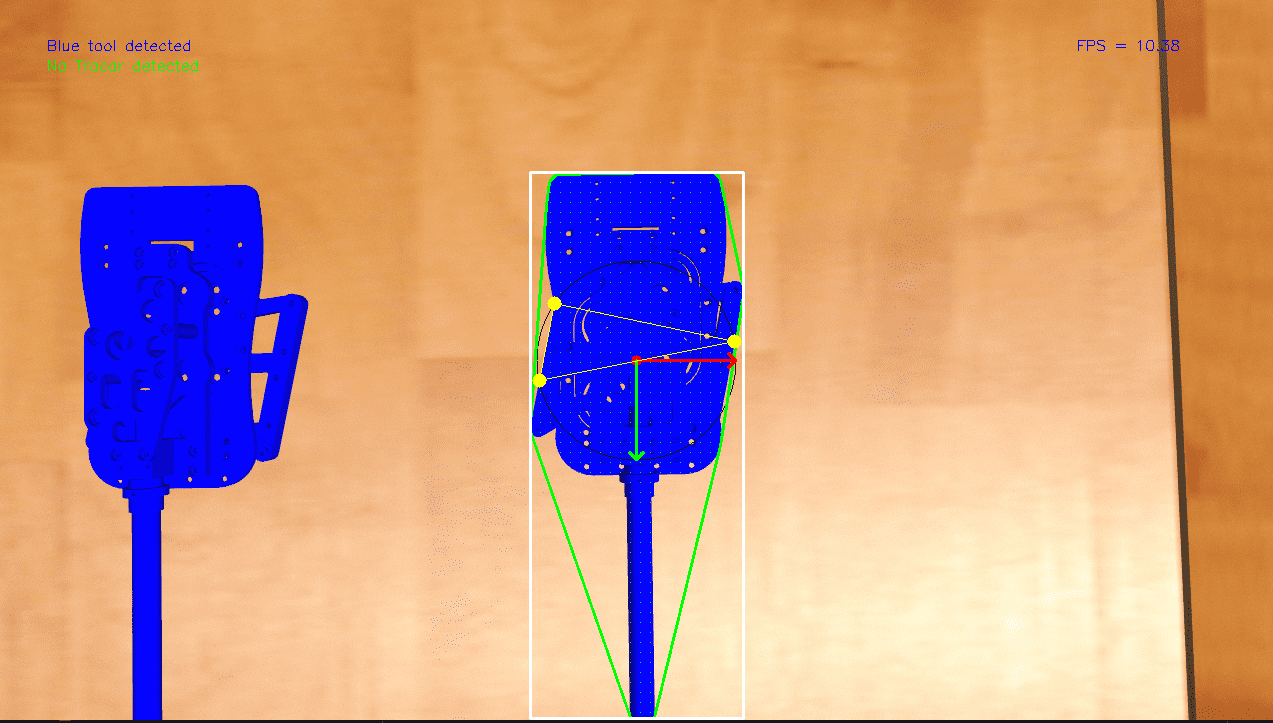
\includegraphics[width=0.6\textwidth]{../images/grasp-points-triangle.png}\\
\caption{Image based visual servoing and calculation of grasp points. The yellow points are the grasp points and the thin black circumscribed circle is the growing circle that was used to calculate them.}
\end{figure}
\end{center}
\end{frame}

\begin{frame}
\begin{center}
\begin{figure}[!htb]
\centering
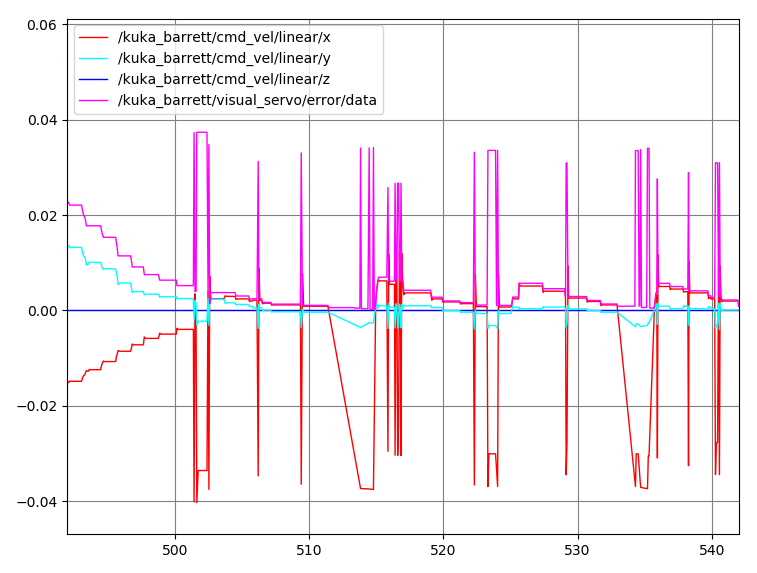
\includegraphics[width=0.45\textwidth]{../images/robot_planner5/visual_servo_controller3.png}
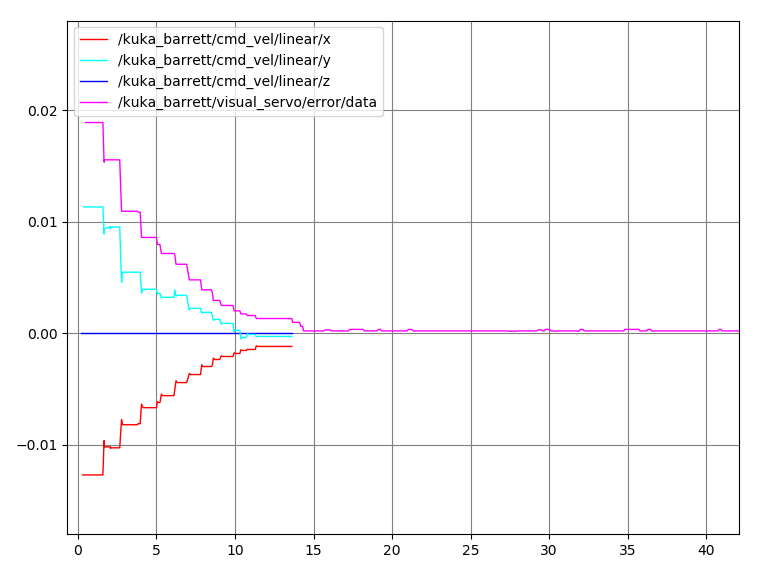
\includegraphics[width=0.45\textwidth]{../images/robot_planner5/visual_servo_controller4.png}\\
\caption{Visual servo controller error diagrams. On the left image in the error graphs appear some spikes. These spikes occur from the sudden temporary detection 
of a nearby surgical tool. On the right image, these spikes are filtered out, and only the error graphs of the visual servoing of one tool are shown. The  
controller parameters are $K_p = 0.9, K_d = 0.2$}
\end{figure}
\end{center}
\end{frame}